\documentclass[20pt]{letter}
\usepackage{amsmath}
\usepackage{amsthm}
\usepackage{amssymb}
\usepackage{fullpage}
\usepackage{graphicx}
\usepackage{geometry}
 \geometry{
 a4paper,
 total={180mm,257mm},
 left=12mm,
 top=20mm,
 }

\newcommand{\abs}[1]{{\left\lvert #1 \right\rvert}}	
\newenvironment{solution}{\textbf{Solution:}}{\hfill$\square$}


\begin{document}

\begin{center}
{\LARGE \textbf{
CS685 - Data Mining\\
2020-2021-I: Assignment 1
}}\end{center}

{\Large
Name: Sarthak Singhal        ~~~~~~~~~~~~~~~~~~~~~~~~~~~~~~~~~~~~~~~~~~~~~~~~~~~~~~~~~~   Roll No.: 170635\\\\}
%If you discuss the question with someone, please mention their name on your assignment. Remember, you are allowed to discuss and not copy.
%You can use any theorem used in the class except if that theorem itself needs to be proven in the question.

%Please print on both sides while submitting the assignment.


% Based on decoding of Reed Solomon codes

\begin{enumerate}
{ \Large
\item \textbf{Question 10}
}
{ \fontsize{13}{13}\selectfont\\\\
%Write your solution here.
The COVID data is considered from 15th March 2020 to 5th September 2020 which comprises of 25 weeks. The below graph shows the number of cases reported in a particular week for overall India.\\
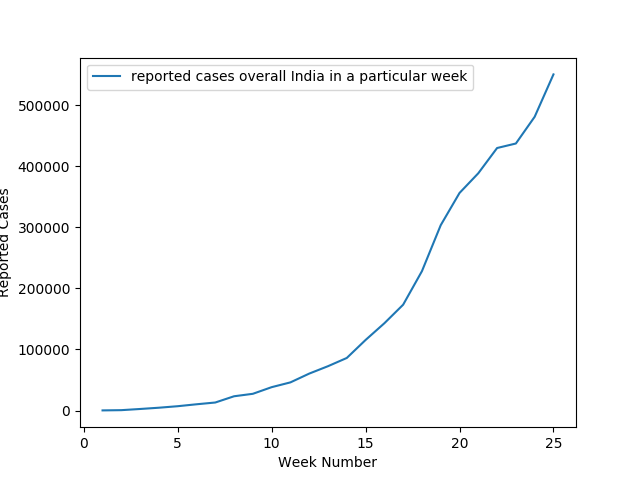
\includegraphics[scale=0.8]{analysis2.png}\\\\
The lockdown 1.0 was from 25-03 to 14-04 i.e. from week 2 to week 4.\\
The lockdown 2.0 was from 15-04 to 03-05 i.e. from week 5 to week 7.\\
The lockdown 3.0 was from 04-05 to 17-05 i.e. from week 8 to week 9.\\
The lockdown 4.0 was from 18-05 to 31-05 i.e. from week 10 to week 11.\\
As we can see from the graph that till the lockdown was imposed the number of cases reported on a per week basis were very low. But we can see that just from week 15 i.e. after completion of lockdown the number of cases have increased drastically with the curve being monotonously increasing. Towards the end more than 5 lakh cases were reported per week.\\\\
There are some districts which have reported more than 1 lakh cases in this period of 25 weeks. Those districts are: Bengaluru urban, Chennai, Delhi, Mumbai, Pune, Thane. Notice that almost all of them are the top metropolitan cities on India which kind of makes it obvious that why they have such large number of cases.\\\\

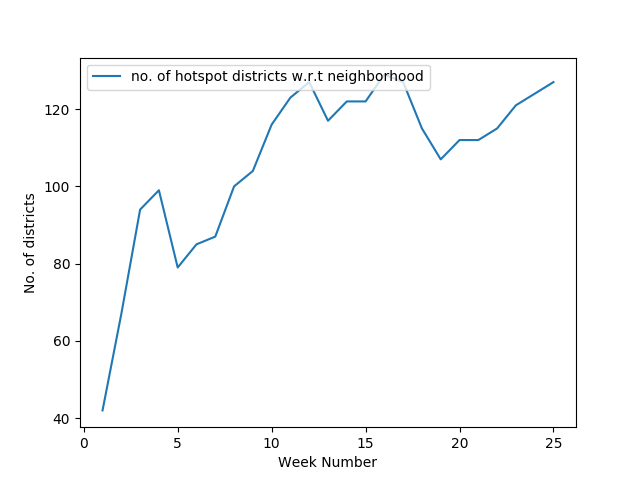
\includegraphics[scale=0.8]{analysis1.png}\\\\
Also, the number of hotspots have increased over the time. In the last week almost $(1/6)^{th}$ of all districts of India have become hotspots.\\
Ahmedabad, Delhi, Bengaluru urban, Surat, Bhopal have been in the top-5 hotspots w.r.t neighborhood for than 9 weeks out of 25.\\
Mahe and Karaikal in Puducherry have been in the top-5 coldspots w.r.t neighborhood for than 11 weeks out of 25.

}

\end{enumerate}

\end{document}


